\documentclass[11pt]{article}
\usepackage{amsmath,amssymb,enumitem,algorithm,algpseudocode}
\usepackage[UTF8]{ctex}
\usepackage[braket]{qcircuit}
\usepackage{graphicx}
\parindent=22pt
\parskip=3pt
\oddsidemargin 18pt \evensidemargin 0pt
\leftmargin 1.5in
\marginparwidth 1in \marginparsep 0pt \headsep 0pt \topskip 20pt
\textheight 225mm \textwidth 148mm
\renewcommand{\baselinestretch}{1.15}
\begin{document}
\title{{\bf 理论作业一 \quad 量子比特与量子门}}
\author{周楠 \quad 3220102535}
\date{\today}
\maketitle

\begin{tabular*}{13cm}{r}
\hline
\end{tabular*}

\vskip 0.3 in

{\bf 1.} 已知双量子比特系统的量子态如下 $|\psi\rangle = \begin{bmatrix} \frac{1}{2} & x & 3x & \frac{i}{2\sqrt{2}} \end{bmatrix} ^ \intercal \in \mathbb{C}^4$ ,求该系统处于 $|01\rangle$ 态的概率。

利用量子态的归一化条件,即整个量子态的概率总和必须等于 1。这意味着态矢量的各个分量的绝对值平方之和必须等于 1。

\[
\left|\frac{1}{2}\right|^2 + |x|^2 + |3x|^2 + \left|\frac{i}{2\sqrt{2}}\right|^2 = 1
\]

\[
\frac{1}{4} + |x|^2 + 9|x|^2 + \frac{1}{8} = 1
\]
\[
10|x|^2 = \frac{5}{8}
\]
\[
|x|^2 = \frac{5}{80} = \frac{1}{16}
\]
因此该系统处于 $|01\rangle$ 态的概率为 \(\dfrac{1}{16}\)。

\vskip 0.3 in

{\bf 2.} 已知单量子比特的态矢量为 $|\psi\rangle = \begin{bmatrix} 3/5 \\ 4/5 \end{bmatrix}$ ,求该量子比特的Bloch球坐标。

$$
|\psi \rangle = \cos(\frac{\theta}{2})|0\rangle + e^{i\phi}\sin(\frac{\theta}{2})|1\rangle 
$$

$$
\cos(\frac{\theta}{2}) = \frac{3}{5}, \quad e^{i\phi}\sin(\frac{\theta}{2}) = \frac{4}{5}
$$

$$
\sin(\frac{\theta}{2}) = \sqrt{1 - \cos^2(\frac{\theta}{2})} = \frac{4}{5}
$$

因此,
$$
e^{i\phi} = 1, \quad \phi = 0, \theta = 2 \cdot arccos(\frac{3}{5})
$$

\vskip 0.3 in

{\bf 3.} Bell 态指双量子比特系统的四个特殊量子态,他们是双量子比特系统中纠缠度最高的量子态,因此也称为最大纠缠态,在量子隐形传态、量子算法中有着广泛的应用。一般而言,Bell 态定义如下:
\begin{align}
    |\beta_{xy}\rangle = \frac{|0y\rangle + (-1)^x|1\bar{y}\rangle}{\sqrt{2}}, \quad x,y \in \{0,1\}, \quad \bar{y} = 1-y
\end{align}
\begin{enumerate}[label=\alph*.]
\item 证明 Bell 态是纠缠态。

如果一个态不能表示为两个单量子比特的直接积形式,则它是纠缠态。
\begin{enumerate}
    \item \(|\beta_{00}\rangle = \frac{1}{\sqrt{2}} (|00\rangle + |11\rangle)\)
    \item \(|\beta_{01}\rangle = \frac{1}{\sqrt{2}} (|01\rangle + |10\rangle)\)
    \item \(|\beta_{10}\rangle = \frac{1}{\sqrt{2}} (|00\rangle - |11\rangle)\)
    \item \(|\beta_{11}\rangle = \frac{1}{\sqrt{2}} (|01\rangle - |10\rangle)\)
\end{enumerate}
我们逐个检查这四个 Bell 态,看看它们能否表示为单量子比特态的张量积。显然上述Bell态无法进行分解。

以 $\beta_{00}$ 为例:如果测量第一个量子比特的状态为 $|0\rangle$,那么第二个量子比特的状态必定为 $|0\rangle$;同样,如果测量第一个量子比特的状态为 $|1\rangle$,那么第二个量子比特的状态也必定为 $|1\rangle$。

\item 用 H、X、Z 和 CNOT 门设计四个量子电路,使得初态为 $|00\rangle$ 的双量子比特系统经这些量子电路作用后分别演化为四个 Bell 态。
\begin{enumerate}
    \item \(|\beta_{00}\rangle = \frac{1}{\sqrt{2}} (|00\rangle + |11\rangle)\)
    
    1. 对第一个量子比特应用 Hadamard 门:\(H\)。

    2. 对两个量子比特应用 CNOT 门,第一个比特为控制比特,第二个为目标比特。
    $$
    \begin{bmatrix} 1 & 1 \\ 1 & -1 \end{bmatrix} |00\rangle = \begin{bmatrix} 1 & 1 \\ 1 & -1 \end{bmatrix} |0\rangle |0\rangle = \frac{|00\rangle + |10\rangle}{\sqrt 2} 
    $$
    $$
    \text{CNOT} \frac{|00\rangle + |10\rangle}{\sqrt 2}  = \frac{|00\rangle + |11\rangle}{\sqrt 2}
    $$
    对应的电路图为:
    \[ \Qcircuit @C=1.0em @R=1.5em {
    \lstick{q_0} & \gate{H} & \ctrl{1}  & \qw \\
    \lstick{q_1} & \qw & \targ  & \qw 
    } \]
    \newpage
    \item \(|\beta_{01}\rangle = \frac{1}{\sqrt{2}} (|01\rangle + |10\rangle)\)
    
    1. 对第一个量子比特应用 Hadamard 门 

    2. 对第二个量子比特应用 X 门(NOT 门)。

    3. 对两个量子比特应用 CNOT 门,第一个比特为控制比特,第二个为目标比特。
    $$
    \begin{bmatrix} 1 & 1 \\ 1 & -1 \end{bmatrix} |00\rangle = \begin{bmatrix} 1 & 1 \\ 1 & -1 \end{bmatrix} |0\rangle |0\rangle = \frac{|00\rangle + |10\rangle}{\sqrt 2} 
    $$
    $$
    X \frac{|00\rangle + |10\rangle}{\sqrt 2}  = \frac{|01\rangle + |11\rangle}{\sqrt 2}
    $$
    $$
    \text{CNOT} \frac{|01\rangle + |11\rangle}{\sqrt 2}  = \frac{|01\rangle + |10\rangle}{\sqrt 2}
    $$
    对应的电路图为:
    \[ \Qcircuit @C=1.0em @R=1.5em {
    \lstick{q_0} & \gate{H} & \ctrl{1}  & \qw \\
    \lstick{q_1} & \gate X & \targ  & \qw 
    } \]
    \item \(|\beta_{10}\rangle = \frac{1}{\sqrt{2}} (|00\rangle - |11\rangle)\)
    
    1. 对第一个量子比特应用 Hadamard 门

    2. 对第一个量子比特应用 Z 门。

    3. 对两个量子比特应用 CNOT 门,第一个比特为控制比特,第二个为目标比特。
    $$
    \begin{bmatrix} 1 & 1 \\ 1 & -1 \end{bmatrix} |00\rangle = \begin{bmatrix} 1 & 1 \\ 1 & -1 \end{bmatrix} |0\rangle |0\rangle = \frac{|00\rangle + |10\rangle}{\sqrt 2} 
    $$
    $$
    Z \frac{|00\rangle + |10\rangle}{\sqrt 2}  = \frac{|00\rangle - |10\rangle}{\sqrt 2}
    $$
    $$
    \text{CNOT} \frac{|00\rangle - |10\rangle}{\sqrt 2}  = \frac{|00\rangle - |11\rangle}{\sqrt 2}
    $$
    对应的电路图为:
    \[ \Qcircuit @C=1.0em @R=1.5em {
    \lstick{q_0} & \gate{H} & \gate Z  & \ctrl{1}  & \qw \\
    \lstick{q_1} & \qw & \qw & \targ  & \qw 
    } \]
    \newpage
    \item \(|\beta_{11}\rangle = \frac{1}{\sqrt{2}} (|01\rangle - |10\rangle)\)
    
    1. 对第一个量子比特应用 Hadamard 门

    2. 对第二个量子比特应用 X 门(NOT 门)。

    3. 对第一个量子比特应用 Z 门。

    4. 对两个量子比特应用 CNOT 门,第一个比特为控制比特,第二个为目标比特。
    $$
    \begin{bmatrix} 1 & 1 \\ 1 & -1 \end{bmatrix} |00\rangle = \begin{bmatrix} 1 & 1 \\ 1 & -1 \end{bmatrix} |0\rangle |0\rangle = \frac{|00\rangle + |10\rangle}{\sqrt 2}
    $$
    $$
    X \frac{|00\rangle + |10\rangle}{\sqrt 2}  = \frac{|01\rangle + |11\rangle}{\sqrt 2}
    $$
    $$
    Z \frac{|01\rangle + |11\rangle}{\sqrt 2}  = \frac{|01\rangle - |11\rangle}{\sqrt 2}
    $$
    $$
    \text{CNOT} \frac{|01\rangle - |11\rangle}{\sqrt 2}  = \frac{|01\rangle - |10\rangle}{\sqrt 2}
    $$
    对应的电路图为:
    \[ \Qcircuit @C=1.0em @R=1.5em {
    \lstick{q_0} & \gate{H} & \gate Z & \qw & \ctrl{1}  & \qw \\
    \lstick{q_1} & \qw & \gate X & \qw & \targ  & \qw 
    } \]
\end{enumerate}
\end{enumerate}


\vskip 0.3 in

{\bf 4.} 证明下图中的两个量子电路等价。(提示:计算两个量子电路对应的酉矩阵)

\[ \Qcircuit @C=1.0em @R=2.0em {
\lstick{q_0} & \targ & \qw \\
\lstick{q_1} & \ctrl{-1} & \qw
} \]


\[ \Qcircuit @C=1.0em @R=1.5em {
\lstick{q_0} & \gate{H} & \ctrl{1} & \gate{H} & \qw \\
\lstick{q_1} & \gate{H} & \targ & \gate{H} & \qw 
} \]

\begin{enumerate}
    \item 量子电路1:$q_1$ 作为控制位,$q_0$ 作为目标位,对应的酉矩阵为
    $$
    CNOT = |00\rangle \langle 00| + |01\rangle \langle 01| + |10\rangle \langle 11| + |11\rangle \langle 10|\\
        = \begin{bmatrix} 1 & 0 & 0 & 0 \\ 0 & 1 & 0 & 0 \\ 0 & 0 & 0 & 1 \\ 0 & 0 & 1 & 0 \end{bmatrix}
    $$
    \newpage
    \item 量子电路2:
    \begin{enumerate}
        \item 1. 对 $q_0$ 和 $q_1$ 应用 Hadamard 门 \(H\)。
        \[
        H \otimes H = \frac{1}{2} \begin{bmatrix} 
        1 & 1 & 1 & 1 \\ 
        1 & -1 & 1 & -1 \\ 
        1 & 1 & -1 & -1 \\ 
        1 & -1 & -1 & 1 
        \end{bmatrix}
        \]
        \item 2. 对 $q_0$ 作为控制位,$q_1$ 作为目标位应用 CNOT 门。
        \[
        CNOT = \begin{bmatrix} 
        1 & 0 & 0 & 0 \\ 
        0 & 0 & 0 & 1 \\ 
        0 & 0 & 1 & 0 \\ 
        0 & 1 & 0 & 0 
        \end{bmatrix}
        \]
        \item 3. 再次对 $q_0$ 和 $q_1$ 应用 Hadamard 门 \(H\)。

        \[
        U = (H \otimes H) \cdot CNOT \cdot (H \otimes H)
          = \frac{1}{4} \cdot \begin{bmatrix}
            1 & 1 & 1 & 1 \\ 
            1 & -1 & 1 & -1 \\ 
            1 & 1 & -1 & -1 \\ 
            1 & -1 & -1 & 1 
            \end{bmatrix} 
            \cdot
            \begin{bmatrix} 
            1 & 0 & 0 & 0 \\ 
            0 & 0 & 0 & 1 \\ 
            0 & 0 & 1 & 0 \\ 
            0 & 1 & 0 & 0 
            \end{bmatrix}
            \cdot
            \begin{bmatrix}
            1 & 1 & 1 & 1 \\ 
            1 & -1 & 1 & -1 \\ 
            1 & 1 & -1 & -1 \\ 
            1 & -1 & -1 & 1 
            \end{bmatrix}
        \]
        \[
            U = (H \otimes H) \cdot CNOT \cdot (H \otimes H)
            = \dfrac{1}{4}
            \begin{bmatrix}
                4 & 0 & 0 & 0 \\
                0 & 4 & 0 & 0 \\
                0 & 0 & 0 & 4 \\
                0 & 0 & 4 & 0
            \end{bmatrix}
            = \begin{bmatrix}
                1 & 0 & 0 & 0 \\
                0 & 1 & 0 & 0 \\
                0 & 0 & 0 & 1 \\
                0 & 0 & 1 & 0
            \end{bmatrix}
        \]
    \end{enumerate}

\end{enumerate}


\vskip 0.3 in
\newpage
{\bf 5.} 证明厄米算符 $A$ 的任一本征值均为实数,且不同本征值对应的本征态正交。

\begin{figure}[H]
    \centering
    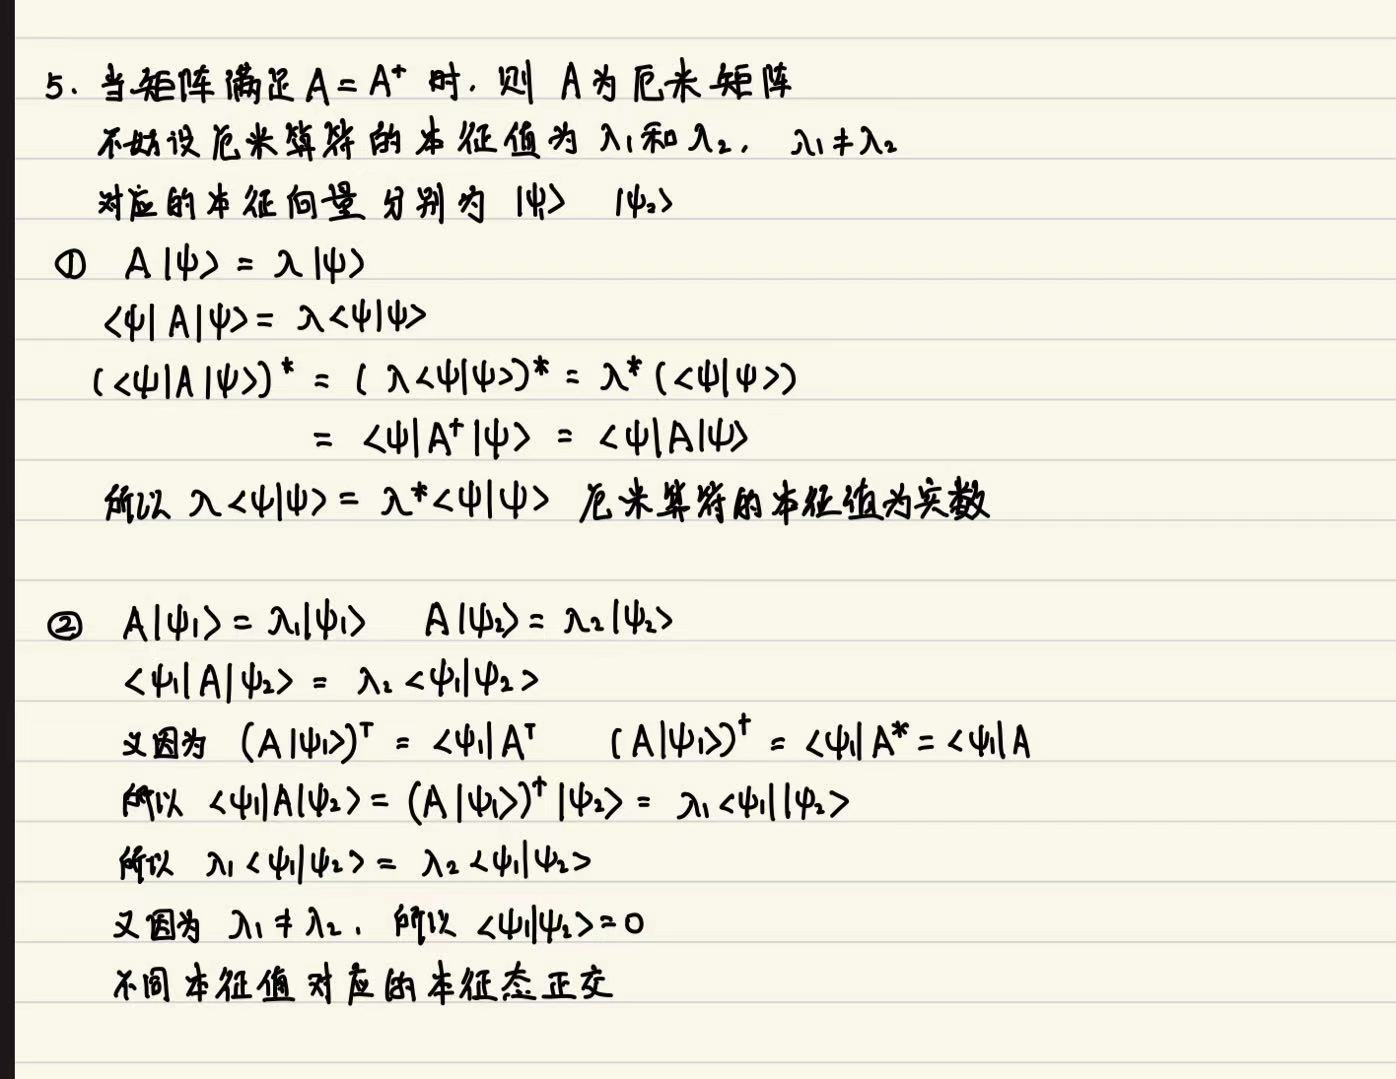
\includegraphics[width=0.8\textwidth]{1.jpg}
\end{figure}

\vskip 0.3 in
{\bf 6.} Deutsch 算法展示了量子计算机强大的并行计算能力。Deutsch-Jozsa 算法是其推广形式,将可分类的函数推广至多比特情形。

已知函数 $f:\{0,1\}^n \rightarrow \{0,1\}$,该函数是常数函数(对所有输入均输出 $0$ ,或对所有输入均输出 $1$)或平衡函数(对恰好一半的输入输出 $0$ ,对另一半输入输出 $1$)。Deutsch-Jozsa 算法只需对实现函数 $f$ 的结构进行一次查询,即可判断 $f$ 是常数函数还是平衡函数。

下图是实现 Deutsch-Jozsa 算法的量子线路。其中,$U_f:|x,y\rangle \to |x,y\oplus f(x)\rangle$ 是实现函数 $f$ 的 $n+1$ 比特的量子门。

\[ \Qcircuit @C=1.0em @R=.7em {
\lstick{\ket{0}} & {/^n} \qw & \gate{H^{\otimes n}} & \multigate{1} {U_f} & \gate{H^{\otimes n}} & \meter & \qw \\
\lstick{\ket{1}} & \qw & \gate{H} & \ghost{U_f} & \qw & \qw & \qw \\
} \]

推导该量子电路中量子态的演化过程,并说明如何基于测量结果判断 $f$ 是常数函数还是平衡函数。(提示:计算 $f$ 为常数函数或平衡函数时的测量结果)


\begin{enumerate}
    \item 初始状态
    假设我们有一个 $n$ 比特的初始量子态 $\ket{0}^{\otimes n}$ 和一个辅助比特 $\ket{1}$,整个系统的初始状态可以写为:
    \[
    \ket{\psi_0} = \ket{0}^{\otimes n} \otimes \ket{1}
    \]
    \item 第一步:Hadamard 变换
    对所有比特应用 Hadamard 门($H^{\otimes n}$ 和 $H$),作用后的状态为:
    \[
    \ket{\psi_1} = \left( \frac{1}{\sqrt{2^n}} \sum_{x \in \{0,1\}^n}\ket{x} \right) \otimes \frac{\left( \ket{0} - \ket{1} \right)}{\sqrt{2}} 
    \]
    其中,$\sum_{x=0}^{2^n-1} \ket{x}$ 表示所有可能的 $n$ 比特组合的叠加态。
    \item 第二步:应用 $U_f$ 门
    接下来,将状态输入到函数门 $U_f$,它的作用是将 $\ket{x, y}$ 变换为 $\ket{x, y \oplus f(x)}$。在我们的状态上应用 $U_f$ 后,量子态变为:
    \[
    \ket{\psi_2} = \frac{1}{\sqrt{2^n}} \sum_{x \in \{0,1\}^n} \ket{x} \otimes |y \oplus f(x)| = \frac{1}{\sqrt{2^n}} \sum_{x=0}^{2^n-1} \ket{x} \otimes (-1)^{f(x)} \frac{1}{\sqrt2} \left( \ket{0} - \ket{1} \right)
    \]
    因此,上述量子态可以进一步简化为:
    \[
    \ket{\psi_2} = \frac{1}{\sqrt{2^n}} \sum_{x \in \{0,1\}^n} (-1)^{f(x)} \ket{x} \otimes \frac{1}{\sqrt{2}} \left( \ket{0} - \ket{1} \right)
    \]
    \item 第三步:再次应用 Hadamard 变换
    
    对于单个量子比特 $x_1$
    \[
        H x_1 = \frac{\sum_{z \in \{0,1\}} (-1)^{xz} \ket{z}}{\sqrt2}
    \]
    对前 $n$ 个比特再次应用 Hadamard 变换,量子态演化为:
    \[
    \ket{\psi_3} = \frac{1}{2^n} \sum_{x \in \{0,1\}^n} \sum_{z \in \{0,1\}^n} (-1)^{f(x) \oplus x \cdot z} \ket{z} \otimes \frac{1}{\sqrt{2}} \left( \ket{0} - \ket{1} \right)
    \]
    其中 $x \cdot z$ 表示 $x$ 和 $z$ 的二进制内积,即 $x \cdot z = x_0z_0 + x_1z_1 + \cdots + x_{n-1}z_{n-1}$。

    \item 第四步:测量前 $n$ 个比特

    $\ket{0} ^{\oplus n}$的概率为:$\langle \psi_3 | 0 \rangle \langle 0 | \psi_3\rangle = (\frac{1}{2^n} \sum_{x \in \{0,1\}^n}  (-1)^{f(x)})^2$
    因为因为除了$\ket{0}$以外的$\ket{z}$都和$\ket{0}$垂直,内积是0,所以其他项都没了,只剩下$\ket{z} = \ket{0}$的这一项。
    \begin{itemize}
        \item 如果f(X)为常数函数,所有的f(x) = 0 或者 1,所有$(-1)^{f(x)}$都相等,平方后得到结果1,测出$\ket{0} ^{\oplus n}$的概率为1
        \item 如果f(x)为平衡函数,一半的$(-1)^{f(x)} = 1$,一半的$(-1)^{f(x)} = -1$,测出$\ket{0} ^{\oplus n}$的概率为0.
    \end{itemize}
    

\end{enumerate}














\end{document}
